\section{Predictors}

We now outline the predictors used to measure the degree of \textbf{social} and \textbf{linguistic} dissemination in the growth and decline words.

\subsection{Social dissemination}

We rely on the dissemination metric proposed by~\newcite{altmann2011} to measure the degree to which a word occupies a specific social niche (e.g., low dissemination implies limited niche).
%Low dissemination implies that a word occupies a limited niche, while a high dissemination implies wide-scale social acceptance. 
%% why is this here?
%A lower user dissemination score indicates that the word was used by fewer users than expected.
%, where we assume the ``expected'' count derives from an underlying Poisson distribution. 
%We compute the dissemination of words across a particular social variable (user, thread, and subreddit) as follows. 
To compute user dissemination $D^U$ for word $w$ at time $t$, we first compute the number of individual users who used word $w$ at time $t$, written $U^{(w)}_t$. 
We then compare this with the expectation $\tilde{U}^{(w)}_t$ under a model in which word frequency is identical across all users.
The user dissemination is the log ratio,
\begin{equation}
%D^{U, w}=\log(\frac{U_{t}^{w}}{\tilde{U}_{t}^{w}}) = \log(U^{w}_{t}) - \log(\tilde{U}^{w}_{t})
\log \frac{U_{t}^{(w)}}{\tilde{U}_{t}^{(w)}} = \log U^{(w)}_{t} - \log \tilde{U}^{(w)}_{t}.
\end{equation}
%The log-ratio is used instead of the raw ratio in parallel with the log-ratio used in the calculation of linguistic niche (see Section \ref{sec:linguistic_dissemination}).

Following \newcite{altmann2011}, the expected count $\tilde{U}_t^{(w)}$ is computed as,
\begin{equation}
\tilde{U}_{t}^{(w)} = \sum_{u \in \mathcal{U}_{t}}(1 - e^{-f_{t}^{(w)}m_{t}^{(u)}}),
\end{equation}
where $m_{t}^{(u)}$ equals the total number of words contributed by user $u$ in month $t$, and $\mathcal{U}_{t}$ is the set of all users active in month $t$. 
This corresponds to a model in which each token from a user has identical likelihood $f_t^{(w)}$ of being word $w$.
%where $f_{t}^{(w)}$ equals the normalized frequency of word $w$ and $m_{t}^{u}$ equals the total number of words contributed by user $u$ in month $t$. 
In this way, we compute dissemination for all users ($D^{U}$), subreddits ($D^{S}$) and threads ($D^{T}$) for each month $t \in \{1 ... T\}$.

%\begin{figure*}
%\centering
%\begin{subfigure}[b]{0.3\textwidth}
%\includegraphics[width=\textwidth]{figures/user_dissemination_annotated.png}
%\end{subfigure}
%\begin{subfigure}[b]{0.3\textwidth}
%\includegraphics[width=\textwidth]{figures/subreddit_dissemination_annotated.png}
%\end{subfigure}
%\begin{subfigure}[b]{0.3\textwidth}
%\includegraphics[width=\textwidth]{figures/thread_dissemination_annotated.png}
%\end{subfigure}
%\caption{Distribution of dissemination values for users ($D^{U}$), subreddits ($D^{S}$), and discussion threads ($D^{T}$). }
%\label{fig:dissemination_annotated}
%\end{figure*}

%We show a comparison between frequency and dissemination in Figure~\ref{fig:dissemination_freq}. 
%The user and thread dissemination values remain consistent for most low frequency words and then grow sharply with higher higher frequency, while the subreddit dissemination values increase steadily with frequency. 
%This division indicates that most rare words are used by roughly the same proportion of users, a similar finding to~\newcite{altmann2011}.
%
%\begin{figure*}[t!]
%\centering
%\includegraphics[width=0.9\textwidth]{figures/dissemination_frequency.png}
%\caption{Example of frequency compared to user, subreddit and thread dissemination. Blue lines indicate median dissemination values, and red lines indicate the 10th and 90th percentile values. Note that all dissemination values tend to be stable across the lower frequencies and only increase significantly in higher frequencies.}
%\label{fig:dissemination_freq}
%\end{figure*}

%Examples of words with high and low average social dissemination are shown in \autoref{tab:predictor-example-words}.
%Highly disseminated words among users include the acronym \example{asap}, a widely accepted form of \example{as soon as possible}, while low-dissemination words among subreddits include \example{crit} (\gloss{critical hit}), which is restricted to users interested in video games.
%Similarly, $D^{T}$ approximates the spread of a word among discussion threads, which is relevant to words such as \example{pvp} (\gloss{player versus player}), an acronym restricted to video game threads.

\subsection{Linguistic dissemination}
\label{sec:linguistic_dissemination}

Linguistic dissemination captures the diversity of linguistic contexts in which a word appears, as measured by unique $n$-gram counts.
%For example, in the sentence \example{that's cool af haha}, the word \example{af} appears in two unique bigrams, \example{cool af} and \example{af haha}. 
We compute the log count of unique trigram\footnote{Pilot analysis with bigram contexts gave similar results.} contexts for all words ($C^{3}$) using all possible trigram positions: in the sentence ``\example{that's cool af haha}'', the term \example{af} appears in three unique trigrams, \example{that's cool af, cool af haha, af haha <END>}.

%We compute the unique count of bigram ($\mathcal{U}^{2}$) and trigram ($\mathcal{U}^{3}$) contexts, and for trigrams we count all possible contexts: in the sentence \example{that's cool af haha}, \example{af} appears in three unique trigrams, \example{that's cool af, cool af haha, af haha <END>}. 
The unique log number of trigram contexts is strongly correlated with log word frequency ($\rho(C^{3}, f) = 0.904$), as implied by Heaps' law~\cite{egghe2007}.
We therefore adjust this statistic by comparing with its expected value $\tilde{C}^{3}$.
%(coefficient of determination $R^{2}(\mathcal{U}^{2}, f) = 0.781, R^{2}(\mathcal{U}^{3}, f) = 0.904$), as more frequent words tend to appear in more contexts. 
At each timestep $t$, we fit a linear regression between log-frequency and log-unique $n$-gram counts, and then compute the residual between the observed log count of unique trigrams and its expectation, $D^{L} = C^{3}_t - \tilde{C}^{3}_t$.
%The expected log-count $\tilde{C}^{(w)}_t$ is predicted by a linear regression from log-frequency. 
%This follows from the observation that the relationship between word frequency and contexts follows a roughly log-log relationship, similar to Heaps' law~\cite{egghe2007}. 
The residual $D^{L}$, or \emph{linguistic dissemination}, identifies words with a higher or lower number of lexical contexts than expected.

\begin{figure}[t!]
\centering
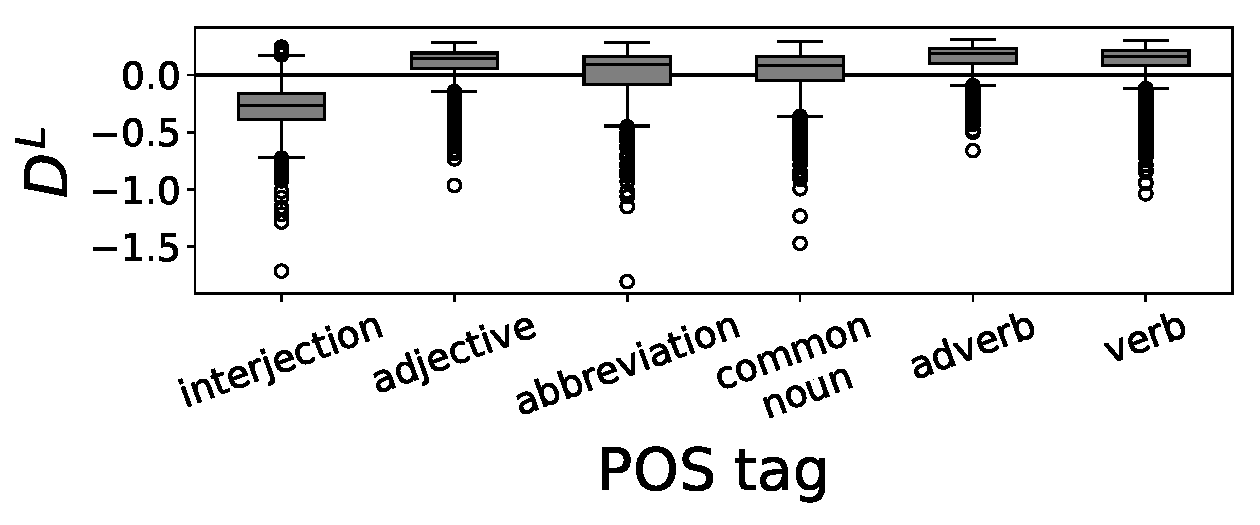
\includegraphics[width=\columnwidth]{figures/pos_DL_distribution.pdf}
\caption{Distribution of mean linguistic dissemination ($D^{L}$) across part of speech groups.}
\label{fig:pos-cd-dist}
% scripts/frequency/plot_pos_DL_distribution.py
\end{figure}

Linguistic dissemination can separate words by grammatical category, as shown in \autoref{fig:pos-cd-dist} where the mean $D^{L}$ values are computed for words across common part-of-speech categories.
Part-of-speech tags were computed over the entire corpus using a Twitter-based tagger~\cite{gimpel2011}, and each word type was assigned the most likely POS tag to provide an approximate distribution of tags over the vocabulary.
Interjections have a lower median $D^{L}$ than other word categories due to the tendency of interjections to occur in limited lexical contexts.
Conversely, verbs have  a higher median $D^{L}$ due to the flexibility of verbs' arguments (e.g., subject and object may both be open-class nouns).

%Examples of growth words with high and low linguistic dissemination are shown in \autoref{tab:predictor-example-words}. 
%High dissemination words include flexible acronyms (\example{aka}) and modifiers that can apply to a variety of contexts (\example{ish}).
%Words with low linguistic dissemination include words that are often used in sentence initial or final position (\example{yikes}).
%, and more topic-specific words (\example{ooc}, \gloss{out of character}). 
%These differences are due in part to the grammatical aspects of linguistic dissemination: for instance, adjectives (\example{ingame}) tend to have higher context diversity than interjections (\example{yeah}). 

%\paragraph{Grammatical aspects of linguistic dissemination} 
%To confirm the grammatical aspects captured by linguistic dissemination, we visualize the distribution of $D^{L}$ values across words grouped by part of speech tags.
%%The grammatical aspects of linguistic linguistic dissemination are confirmed with the distribution of $D^{L}$ across part of speech tags. 
%These tags were obtained automatically from the CMU Twitter Part-of-Speech tagger~\cite{gimpel2011}.\footnote{\url{https://github.com/brendano/ark-tweet-nlp} (Accessed 17 June 2017).}
%As shown in \autoref{fig:pos-cd-dist}, interjections have lower linguistic dissemination, which follows from being restricted to sentence-initial or sentence-final position. 
%In contrast, adjectives and adverbs have high linguistic dissemination because they can appear throughout the sentence, often near open-class words such as nouns and verbs. 
%But while these differences are real and in some cases substantial (one-way ANOVA between part-of-speech groups: $F=822.6, p < 0.0001$), robustness checks in ~\autoref{sec:results-binary-predict} show that the role of linguistic dissemination in explaining word growth goes beyond part-of-speech category.
% ANOVA results: output/tag_vs_DC_ANOVA.tsv
%Some part of speech groups such as proper nouns have lower bigram context diversity than trigram context diversity, which may reflect how proper nouns in English often occur in pairs (e.g. \example{Hillary Clinton}) and have more restricted bigram contexts than trigram contexts.
%interjections tend to have a less diverse trigram context (e.g. \emph{omg} often followed by multiple exclamation points).
%Bigram context diversity also has larger variance in nearly all part of speech categories as compared to trigram context diversity, which demonstrates that short-term dependencies (bigrams) are less predictable than long-term dependencies (trigrams).
%We find that bigram and trigram context diversity are highly collinear ($R=0.91$), and we choose to include only trigram diversity in our experiments. \ian{not sure if this is enough justification}

%we use this metric to approximate the linguistic factors that influence the adoption of a lexical innovation. 
% diversity to find words with an unexpectedly high number of bigram and trigram context counts, we can approximate the semantic diversity of lexical innovations as a proxy for linguistic context to contrast with the social context (dissemination).

%\ian{should we show examples of $C^{2}$ and $C^{3}$ disagreeing? e.g. where a word has high $C^{3}$ and low $C^{2}$.}

%Following prior work in quantifying polysemy~\cite{hamilton2016change}, we use the embeddings computed at each timestep to build a network of related words. We connect two words $w_{i}$ and $w_{j}$ with an edge if $w_{j}$ is one of the $k$-nearest neighbors of $w_{i}$, determined by cosine distance between the embeddings. We set $k=10$ \ian{through experimentation?}. For each word in the network, we then compute the clustering coefficient
